\documentclass[reqno,a4paper,12pt]{amsart}

\usepackage{amsmath,amssymb,amsthm,geometry,xcolor,soul,graphicx}
\usepackage{titlesec}
\usepackage{enumerate}
\usepackage{lipsum}
\usepackage{listings}
%\RequirePackage[most]{tcolorbox}
\usepackage{braket}
\allowdisplaybreaks[4] %align公式跨页
\usepackage{xeCJK}
\setCJKmainfont[AutoFakeBold = true]{Kai}
\geometry{left=0.7in, right=0.7in, top=1in, bottom=1in}

\renewcommand{\baselinestretch}{1.3}

\title{介观物理第十一次作业}
\author{董建宇 ~~ 202328000807038}

\begin{document}

\maketitle
\titleformat{\section}[hang]{\small}{\thesection}{0.8em}{}{}
\titleformat{\subsection}[hang]{\small}{\thesubsection}{0.8em}{}{}

\textbf{Problem III.7} Verify Eq. (220).
\[
	T_{12} = \frac{T_1T_2}{1+R_1R_2-2\sqrt{R_1R_2}\cos\theta}. \tag{220}
\]

\begin{proof}
根据式(219),有:
\[
	D = \frac{e^{i\phi} t_1t_2}{1-e^{2i\phi} r_2r_1'}.
\]

则透射率为:
\[
	T_{12} = \vert D \vert^2 = \frac{T_1T_2}{(1-e^{2i\phi} r_2r_1')(1-e^{-2i\phi} r_2^*{r_1^*}')} = \frac{T_1T_2}{1 + R_1'R_2 - 2\sqrt{R_1'R_2}\cos\theta}.
\]

其中
\[
	\theta = 2\phi + \arg(r_2r_1').
\]
\end{proof}


\textbf{Problem III.8} Find proper conditions under which $T=1$ in Eq. (238). Note that the $2\times 2$ scattering matrix
\[
	S_i = \left( \begin{matrix}
		r_1 & t_i' \\
		t_i & r_i'
	\end{matrix} \right)
\]

must be a unitary matrix, where $i=1,2$.
\[
	T = \frac{4\vert A \vert^2}{\vert C \vert^2} = \frac{4\vert t_2 (r_1-1) (1-r_1') \vert^2}{\vert t_2^2 - (2-r_1-r_2)(2-r_1'-r_2') \vert^2}. \tag{238}
\]

\begin{proof}
散射矩阵$S_i$满足
\[
	S_i^\dagger S_i = S_i S_i^\dagger = \mathbf{I}; \ \vert r_i \vert^2 + \vert t_i \vert^2 = 1; \ \vert r_i' \vert^2 + \vert t_i' \vert^2 = 1; \ r_it_i'^* + t_ir_i'^* = 0.
\]

要求$T=1, \ t_1=0$,则有$\vert r_1 \vert = \vert r_1' \vert = 1$,则$r_1$和$r_1'$可以写作:
\[
	r_1 = e^{i\theta_1}, \ r_1' = e^{i\theta_2}, \ t_1 = t_1' = 0; \ r_2 = r e^{i\theta_2}, \ r_2' = r e^{i\theta_2'}, \ t_2 = t_2' = t e^{i\varphi}.
\]

利用$\vert r_2 \vert^2 + \vert t_2 \vert^2 = r^2 + t^2 = 1$,可以将$r_2, t_2$重新写作:
\[
	r_2 = \cos\alpha e^{i\theta_2}, \ r_2' = \cos\alpha e^{i\theta_2'}; \ t_2 = t_2' = \sin\alpha e^{i\varphi} = -i\sin\alpha \sqrt{r_2r_2'}.
\]

其中,利用了$\varphi = \frac{1}{2}(\theta_2 + \theta_2' - \pi)$。当$T = 1$时,有:
\[
	4\vert t_2(r_1-1)(1-r_1') \vert^2 = \vert t_2^2 - (2-r_1-r_2)(2-r_1'-r_2') \vert^2.
\]

根据讲义,$\theta_1$和$\theta_1'$的恰当选取可以使得$T=1$,从而可以选取合适的$\theta_2, \theta_2', \alpha$简化计算。取$\theta_2 = \theta_2' = 0,\ \alpha = \frac{\pi}{2}$。则有:
\[
	r_2 = r_2' = 0; \ t_2 = t_2' = -i.
\]

则$T=1$得:
\[
	4\vert r_1r_1' - r_1 - r_1' + 1 \vert^2 = \vert r_1r_1' - 2(r_1+r_1') + 5 \vert^2.
\]

化简可得:
\[
	r_1r_2' + r_1^*r_1'^* - 4(r_1+r_1^*) - 4(r_1'+r_1'^*) + 18 = 0.
\]

即
\[
	\cos(\theta_1+\theta_1') - 4\cos\theta_1 - 4\cos\theta_1' + 9 = 0.
\]
\end{proof}


\textbf{Problem 3.} 证明贝里相位必定为实数。

\begin{proof}
贝里相位可以写作:
\[
	\gamma(t) = i\int_0^{\mathbf{R}(t)} \bra{n(\mathbf{R})} \nabla_{\mathbf{R}} \ket{n(\mathbf{R})} d\mathbf{R}.
\]

由于微分算符是反厄米算符,可以计算贝里相位共轭为:
\begin{align*}
	\gamma^*(t) =& -i\int_0^{\mathbf{R}(t)}\bra{n(\mathbf{R})} \nabla_{\mathbf{R}} \ket{n(\mathbf{R})}^* d\mathbf{R} \\
	=& -i\int_0^{\mathbf{R}(t)}\bra{n(\mathbf{R})} (\nabla_{\mathbf{R}} )^\dagger \ket{n(\mathbf{R})} d\mathbf{R} \\
	=&i\int_0^{\mathbf{R}(t)}\bra{n(\mathbf{R})} \nabla_{\mathbf{R}} \ket{n(\mathbf{R})} d\mathbf{R} \\
	=& \gamma(t).
\end{align*}

即贝里相位$\gamma(t)$必定为实数。
\end{proof}


\textbf{Problem 4.} 按照下图所示的方式选取石墨烯晶格的基矢,即
\[
	\mathbf{a}_1 = \sqrt{3}a\left( \frac{\sqrt{3}}{2}, \frac{1}{2} \right), \ \ \mathbf{a}_2 = \sqrt{3}a\left( \frac{\sqrt{3}}{2}, -\frac{1}{2} \right),
\]

其中$a$为最近邻原子的间距。利用紧束缚模型,写出只考虑最近邻相互作用的哈密顿量,给出第一布里渊区高对称点$K$和$K'$附近的近似形式,并求解出相应的本征值和本征函数,计算波函数对应的贝里相位;与课堂上给出的结果进行比较,并讨论其异同。

\begin{center}
	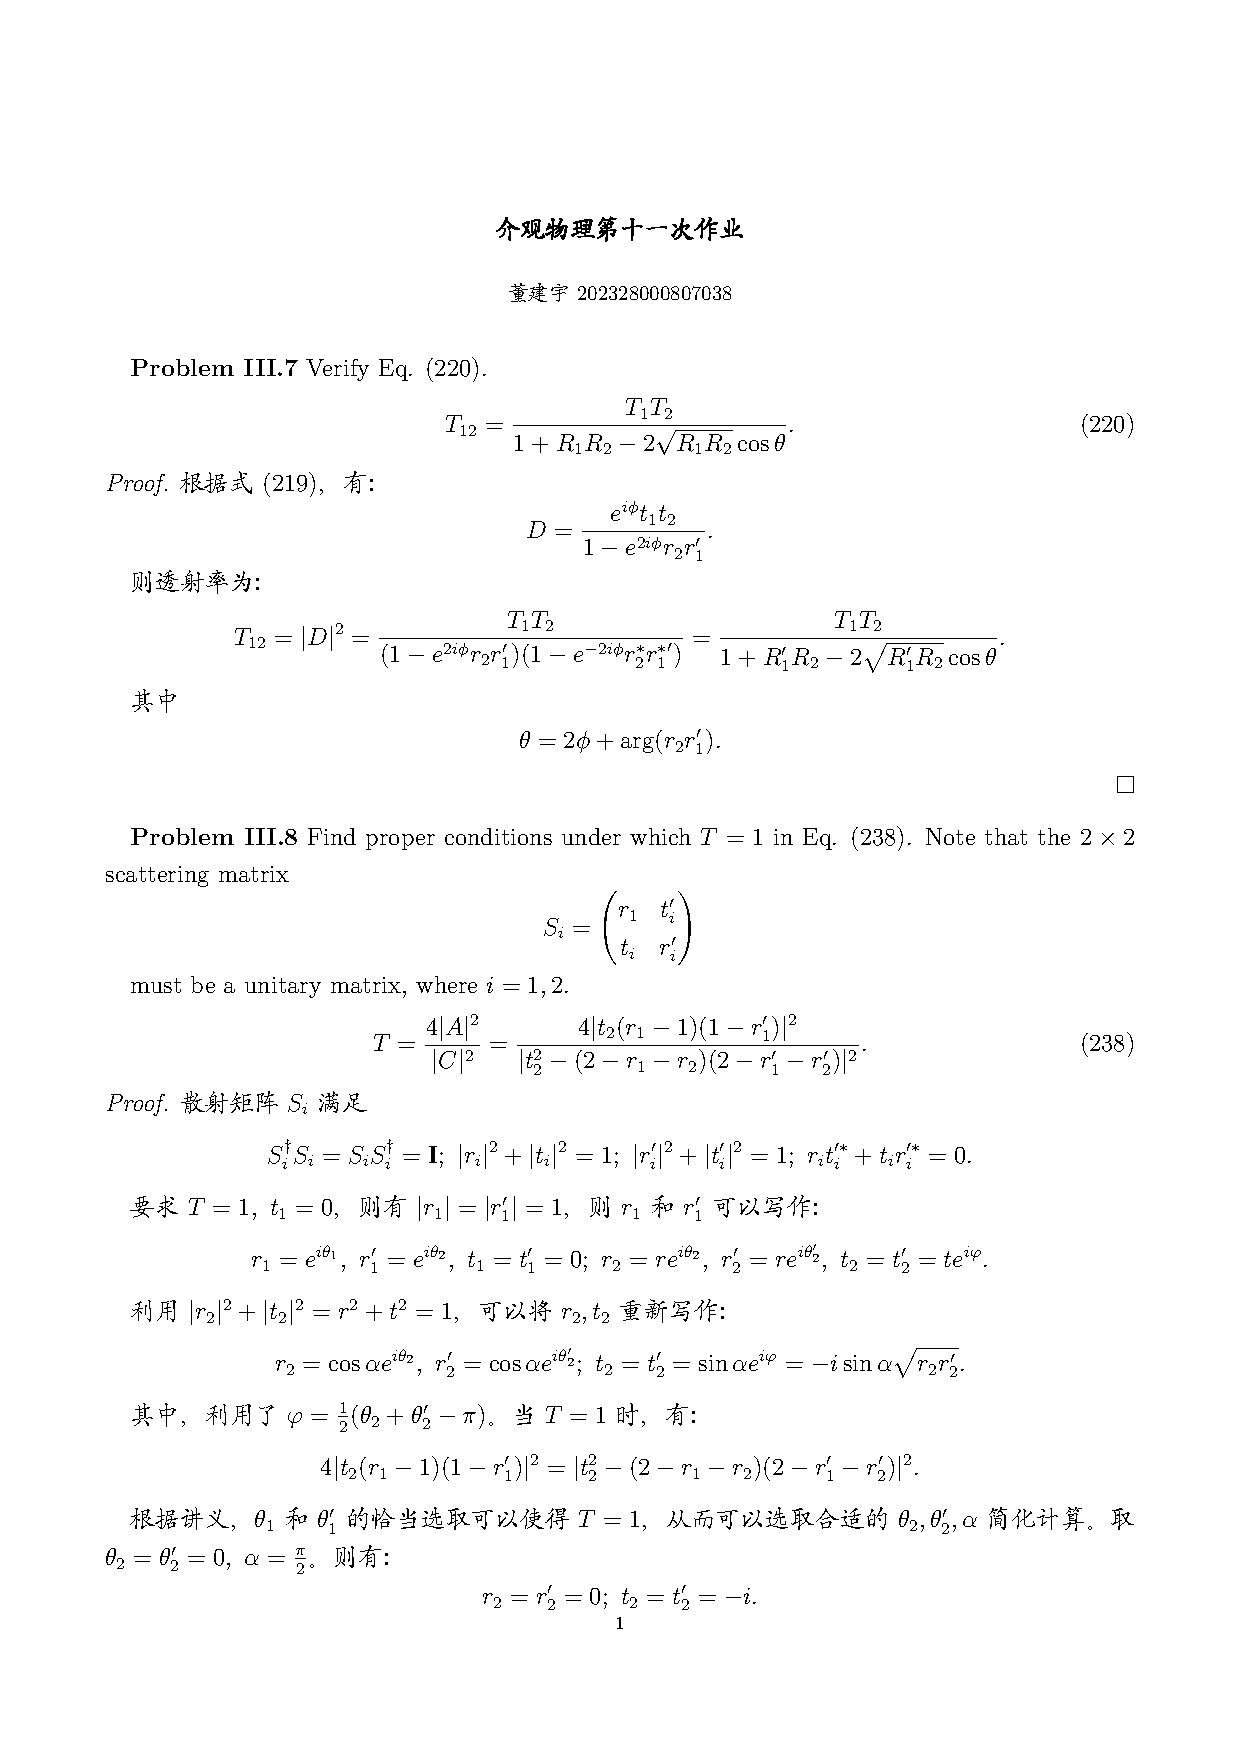
\includegraphics[scale = 0.3]{homework11.jpeg}
\end{center}


\begin{proof}
考虑二次量子化,只考虑近邻相互作用的哈密顿量可以写作:
\[
	\hat{H} = -t\sum_{<i, j> \delta} \hat{a}_i^\dagger \hat{b}_j - t' \sum_i (\hat{a}_i^\dagger \hat{a}_i + \hat{b}_i^\dagger \hat{b}_i) + h.c.
\]

为了简化记号,以下的算符不再写算符记号$\hat{}$,但仍表示算符。两套湮灭算符的展开可以写作:
\[
	a_i = \sum_k a_k e^{-\vec{k} \cdot \vec{r}_i^A}; \ \ b_j = \sum_k b_k e^{i\vec{k} \cdot \vec{r}_j^B}.
\]

则哈密顿量非对角元项可以写作:
\begin{align*}
	\sum_{<i, j>, \vec{\delta}} a^\dagger_i b_j =& \sum_{<i, j>, \vec{\delta}} \sum_k a^\dagger_k e^{-i\vec{k} \cdot \vec{r}_i^A} \sum_{k'} b_{k'} e^{i\vec{k}' \cdot (\vec{r}_i^A + \vec{\delta})} \\
	=& \sum_{kk'} a_k^\dagger b_{k'} \sum_{\vec{\delta}} e^{i\vec{k}' \cdot \vec{\delta}} \sum_i e^{i\vec{r}_i^A \cdot (\vec{k'}-\vec{k})} \\
	=& \sum_{k} a^\dagger_k b_k \sum_{\vec{\delta}} e^{i\vec{k} \cdot \vec{\delta}}.
\end{align*}

其中,在计算过程中忽略了归一化常数$\frac{1}{N}$,但由于$\sum_i e^{i\vec{r}_i^A \cdot (\vec{k'}-\vec{k})} = N \delta(\vec{k} - \vec{k}')$,所以归一化常数被抵消,从而不影响计算结果。

取$t' = 0$,则哈密顿量可以写作:
\[
	H = -t\sum_k \left( \begin{matrix}
		a_k^\dagger & b_k^\dagger
	\end{matrix} \right) \left( \begin{matrix}
		0 & \sum_{\vec{\delta}} e^{i\vec{k} \cdot \vec{\delta}} \\
		\sum_{\vec{\delta}} e^{-i\vec{k} \cdot \vec{\delta}} & 0
	\end{matrix} \right) \left( \begin{matrix}
		a_k \\
		b_k
	\end{matrix} \right)
\]

记
\[
	\vec{H} = (H_x, H_y, H_z).
\]

其中$H_x, H_y, H_z$满足:
\[
	H = -t\sum_k \left( \begin{matrix}
		a_k^\dagger & b_k^\dagger
	\end{matrix} \right) \left( \begin{matrix}
		H_z & H_x-iH_y \\
		H_x+iH_y & H_z
	\end{matrix} \right) \left( \begin{matrix}
		a_k \\
		b_k
	\end{matrix} \right)
\]

结合
\[
	\vec{\delta}_1 = a\left( \frac{1}{2}, \frac{\sqrt{3}}{2} \right); \ \vec{\delta}_2 = a\left( -1, 0 \right); \ \vec{\delta}_1 = a\left( \frac{1}{2}, -\frac{\sqrt{3}}{2} \right);
\]

可以计算:
\begin{align*}
	H_x =& \cos\left[ \frac{a}{2}(k_x + \sqrt{3}k_y) \right] + \cos(ak_x) + \cos\left[ \frac{a}{2}(k_x-\sqrt{3}k_y) \right] \\
	=& \cos(a k_x) + 2\cos(ak_x/2)\cos(\sqrt{3}ak_y/2); \\
	H_y =& \sin(ak_x) - \sin\left[ \frac{a}{2}(k_x + \sqrt{3}k_y) \right] - \sin\left[ \frac{a}{2}(k_x - \sqrt{3}k_y) \right] \\
	=& \sin(ak_x) - 2\sin(ak_x/2)\cos(\sqrt{3}ak_y/2); \\
	H_z =& 0.
\end{align*}

在$K$和$K'$点,倒空间中坐标为:
\[
	K = \left( \frac{2\pi}{3a}, \frac{2\pi}{3\sqrt{3}a} \right); \ K' = \left( \frac{2\pi}{3a}, -\frac{2\pi}{3\sqrt{3}a} \right).
\]

在$K$点的近似形式为:
\begin{align*}
	H_x =& -\frac{1}{2}-\frac{\sqrt{3}}{2}a\delta k_x + 1 -\frac{1}{2}-\frac{\sqrt{3}}{2} \left( \frac{\sqrt{3}}{2}a\delta k_y - \frac{1}{2}a\delta k_x\right) = \frac{3a}{4}(-\sqrt{3}\delta k_x - \delta k_y); \\
	H_y =& \frac{\sqrt{3}}{2}-\frac{1}{2}a\delta k_x - \frac{\sqrt{3}}{2} + \frac{1}{2}\left( \frac{1}{2}a\delta k_x + \frac{\sqrt{3}}{2}a\delta k_y \right) - \frac{1}{2}a(\delta k_x-\sqrt{3}\delta k_y) = \frac{3a}{4} (-\delta k_x + \sqrt{3} \delta k_y); \\
	H_z =& 0.
\end{align*}

本征值为
\[
	\lambda = \pm \vert -t \vec{H} \vert = \pm \frac{3}{2}at\vert \delta \vec{k} \vert.
\]

其中,对哈密顿量的相似变换矩阵为:
\[
	U = \frac{1}{\sqrt{2}} \left( \begin{matrix}
		\frac{H_z - H}{H_x + iH_y} & \frac{H_z + H}{H_x + iH_y} \\
		1 & 1
	\end{matrix} \right).
\]

则两个本征波函数分别为:
\begin{align*}
	\psi_1 = & \left( \begin{matrix}
		\frac{H_z - H}{H_x + iH_y} \\
		1
	\end{matrix} \right); \text{对应本征值} \ \frac{3}{2}at\vert \delta \vec{k} \vert; \\
	\psi_2 = & \left( \begin{matrix}
		\frac{H_z + H}{H_x + iH_y} \\
		1
	\end{matrix} \right); \text{对应本征值} \ -\frac{3}{2}at\vert \delta \vec{k} \vert.
\end{align*}

从而可以计算贝里相位:
\[
	\gamma_1 = \oint i\bra{\psi_1} \nabla_k \ket{\psi_1} \cdot d\vec{l} = -\pi; \ \gamma_2 = \oint i\bra{\psi_2} \nabla_k \ket{\psi_2} \cdot d\vec{l} = -\pi.
\]

类似的对于$K'$点,近似形式为:
\begin{align*}
	H_x =& 1 - \frac{1}{2} - \frac{\sqrt{3}}{2}a\delta k_x - \frac{1}{2} - \frac{\sqrt{3}}{2}\frac{1}{2}a(\delta k_x-\sqrt{3}\delta k_y) = \frac{3}{4}a(-\sqrt{3}\delta k_x + \delta k_y); \\
	H_y =& \frac{\sqrt{3}}{2} - \frac{1}{2}a\delta k_x - \frac{a}{2}(\delta k_x+\sqrt{3}\delta k_y) - \frac{\sqrt{3}}{2} + \frac{1}{2}\frac{a}{2}(\delta k_x-\sqrt{3}\delta k_y) = \frac{3}{4}a(-\delta k_x - \sqrt{3}\delta k_y); \\
	H_z =& 0.
\end{align*}

类似的,本征值为:
\[
	\lambda = \pm \vert -t \vec{H} \vert = \pm \frac{3}{2}at\vert \delta \vec{k} \vert.
\]

其中,对哈密顿量的相似变换矩阵为:
\[
	U = \frac{1}{\sqrt{2}} \left( \begin{matrix}
		\frac{H_z - H}{H_x + iH_y} & \frac{H_z + H}{H_x + iH_y} \\
		1 & 1
	\end{matrix} \right).
\]

则两个本征波函数分别为:
\begin{align*}
	\psi_3 = & \left( \begin{matrix}
		\frac{H_z - H}{H_x + iH_y} \\
		1
	\end{matrix} \right); \text{对应本征值} \ \frac{3}{2}at\vert \delta \vec{k} \vert; \\
	\psi_4 = & \left( \begin{matrix}
		\frac{H_z + H}{H_x + iH_y} \\
		1
	\end{matrix} \right); \text{对应本征值} \ -\frac{3}{2}at\vert \delta \vec{k} \vert.
\end{align*}

从而可以计算贝里相位:
\[
	\gamma_1 = \oint i\bra{\psi_1} \nabla_k \ket{\psi_1} \cdot d\vec{l} = -\pi; \ \gamma_2 = \oint i\bra{\psi_2} \nabla_k \ket{\psi_2} \cdot d\vec{l} = -\pi.
\]

综上所述,与上课结果给出的贝里相位不同,但差值为$2\pi$,所以在物理上等价。
\end{proof}


\end{document}